\begin{savequote}[45mm]
\ascii{Any fool can write code that a computer can understand. Good programmers write code that humans can understand.}
\qauthor{\ascii{- Martin Flower}}
\end{savequote}

\chapter{聚集参数} 
\label{ch:param-collector}

\begin{content}

\end{content}

\section{收集器}

\begin{content}

在之前的测试用例里,在匿名命名空间内引入计数器\ascii{num}。当某个用例被执行时,其\ascii{num++}。操作游离在对象之外的计数器是极为危险的,即使该计数器已经被限制在匿名命名空间内;因为,在其可见的作用域内都有可能被他人修改。

这是一种脆弱的设计,用户需要小心地维护计数器的初始化,也需要用户精细控制计数器累加的时机。一则容易引入不经意的错误,二则让计数器的操作散乱到各个子类覆写的\ascii{runTest}之中。

\subsection{测试用例}

为了消除这个不稳定的设计,这里引入\ascii{TestResult}的抽象,它专门负责计数器维护,及其测试结果收集等职责。重构测试用例,对外暴露\ascii{TestResult::runCount}的查询接口。

\begin{leftbar}
 \begin{c++}[caption={\ttfamily{test/mars/core/TestSuiteSpec.cc}}]
#include <gtest/gtest.h>
#include "mars/core/TestCase.h"
#include "mars/core/TestSuite.h"
#include "mars/core/TestResult.h"

namespace {
  struct TestSuiteSpec : testing::Test {
    void run(::Test& test) {
      test.run(result);
    }

  protected:
    TestResult result;
  };
}

TEST_F(TestSuiteSpec, run_multi_test_cases_using_test_suite) {
  TestSuite suite;
  suite.add(new TestCase);
  suite.add(new TestCase);

  run(suite);

  ASSERT_EQ(2, result.runCount());
}
 \end{c++}
\end{leftbar}

\subsection{实现TestResult}

\ascii{TestResult}维护了一个计数器,负责计数器初始化,累计操作数的职责。

\begin{leftbar}
 \begin{c++}[caption={\ttfamily{include/mars/core/TestResult.h}}]
struct TestResult {
  TestResult();

  void onRun();
  int runCount() const;

private:
  int numOfRuns;
};
 \end{c++}
\end{leftbar}

实现\ascii{TestResult}也较为简单。

\begin{leftbar}
 \begin{c++}[caption={\ttfamily{src/mars/core/TestResult.cc}}]
#include "mars/core/TestResult.h"

TestResult::TestResult() : numOfRuns(0) {
}

void TestResult::onRun() {
  numOfRuns++;
}

int TestResult::runCount() const {
  return numOfRuns;
}
 \end{c++}
\end{leftbar}

\subsection{重构TestCase}

当执行\ascii{TestCase::run}时,通知\ascii{TestResult}累加计数器。为了使得代码具有层次感,提取了\ascii{TestCase::runBare}的子函数,使得\ascii{TestCase::run}的主干更加清晰明了。

在头文件中,提取的\ascii{TestCase::runBare}的子函数声明为\ascii{private}。

\begin{leftbar}
 \begin{c++}[caption={\ttfamily{include/mars/core/TestCase.h}}]
#include "mars/core/Test.h"

struct TestCase : Test {
  using Test::Test;

private:
  void run(TestResult&) override;

private:
  virtual void setUp() {}
  virtual void runTest() {}
  virtual void tearDown() {}

private:
  void runBare();
};
 \end{c++}
\end{leftbar}

在实现文件中,搬迁主干逻辑至\ascii{TestCase::runBare}。

\begin{leftbar}
 \begin{c++}[caption={\ttfamily{src/mars/core/TestCase.cc}}]
#include "mars/core/TestCase.h"
#include "mars/core/TestResult.h"

void TestCase::runBare() {
  setUp();
  runTest();
  tearDown();
}

void TestCase::run(TestResult& result) {
  result.onRun();
  runBare();
}
 \end{c++}
\end{leftbar}

\subsection{重构TestSuite}

重构\ascii{TestSuite::run},每次迭代将\ascii{result}透传给\ascii{Test::run},实现多态调用。

\begin{leftbar}
 \begin{c++}[caption={\ttfamily{src/mars/core/TestSuite.cc}}]
#include "mars/core/TestSuite.h"

// ...

void TestSuite::run(TestResult& result) {
  foreach([&result](auto test) {
    test->run(result);
  });
}
 \end{c++}
\end{leftbar}

至此,测试通过。\ascii{TestResult}扮演了聚集参数的角色,它在运行时收集测试运行的结果。

\begin{figure}[H]
\centering
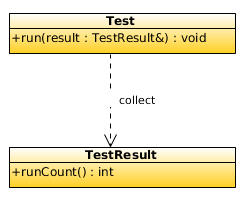
\includegraphics[width=0.4\textwidth]{figures/xunit/test-result.png}
\caption{聚集参数:收集测试结果}
 \label{fig:test-tree}
\end{figure}

\section{统计器}

\ascii{TestResult::runCount}在运行时,通过监听接口统计测试用例的数目。事实上,也可以遍历用例树,直接统计测试用例的数目。构造一个失败的用例,观察如何统计测试用例数目。

\subsection{测试用例}

\begin{leftbar}
 \begin{c++}[caption={\ttfamily{test/mars/core/TestSuiteSpec.cc}}]
#include <gtest/gtest.h>
#include "mars/core/TestCase.h"
#include "mars/core/TestSuite.h"
#include "mars/core/TestResult.h"

namespace {
  struct TestSuiteSpec : testing::Test {
    void run(::Test& test) {
      test.run(result);
    }

    int countTestCases(::Test& test) {
      return test.countTestCases();
    }

  protected:
    TestResult result;
  };
}

TEST_F(TestSuiteSpec, run_multi_test_cases_using_test_suite) {
  TestSuite suite;
  suite.add(new TestCase);
  suite.add(new TestCase);

  run(suite);

  ASSERT_EQ(2, countTestCases(suite));
}
 \end{c++}
\end{leftbar}

\subsection{定义虚接口}

增加\ascii{Test::countTestCases}纯虚接口。

\begin{leftbar}
 \begin{c++}[caption={\ttfamily{include/mars/core/Test.h}}]
#include <string>

struct TestResult;

struct Test {
  explicit Test(const std::string& name = "");
  const std::string& getName() const;

  virtual ~Test() {}
  virtual int countTestCases() const = 0;
  virtual void run(TestResult&) = 0;

private:
  std::string name;
};
 \end{c++}
\end{leftbar}

\subsection{实现虚接口}

\ascii{TestCase::countTestCases}覆写行为直接返回\ascii{1}。

\begin{leftbar}
 \begin{c++}[caption={\ttfamily{src/mars/core/TestCase.cc}}]
int TestCase::countTestCases() const {
  return 1;
}
 \end{c++}
\end{leftbar}

\ascii{TestSuite::countTestCases}覆写行为完成\ascii{reduce}操作。

\begin{leftbar}
 \begin{c++}[caption={\ttfamily{src/mars/core/TestSuite.cc}}]
int TestSuite::countTestCases() const {
  auto num = 0;
  foreach([&num](auto test) {
    num += test->countTestCases();
  });
  return num;
}
 \end{c++}
\end{leftbar}

至此,测试通过。相对于\ascii{TestResult::runCount}通过聚集参数实现用例数目的统计,\ascii{TestResult::countTestCases}更加具有可扩展性;并且,\ascii{TestResult}与\ascii{TestCase}的耦合程度更小。

\end{content}

